%Model Presentation: detailed  presentation of a model, including justifications for design decisions

The presentation of our solution to the \mlpc follows a systematic methodology where modeling choices are introduced step by step, as the requirements are stated. The satisfaction of requirements is explained throughout this presentation.

%\todo[inline]{phrase d'intro pour expliquer que les req étaient couverts au fur et à mesure (côté systématique)}

The designed multilevel architecture shown in Figure~\ref{fig:MultilevelArchitecture} captures the two use cases described in the Process Challenge.

Note that in all following figures, blue is used to represent \FML virtual models and concepts (\textsf{VirtualModel} and \textsf{FlexoConcept} in figure \ref{fig:mm}), see figures \ref{fig:BPMNSubsetExample}, \ref{fig:MultilevelArchitecture}, \ref{fig:LinguisticAndOntologicInstantiation}, \ref{fig:BaseMetamodel}, \ref{fig:AcmeFullArchitecture},  \ref{fig:ToolingArchitecture}, while brown is used for instances of \textsf{FlexoConcept}, see figures \ref{fig:BPMNSubsetExample}, \ref{fig:MultilevelArchitecture}, \ref{fig:LinguisticAndOntologicInstantiation}, \ref{fig:AcmeFullArchitecture},  \ref{fig:ToolingArchitecture}.
% 3, 4, 5, 6, 7, 8, 9
% Expliquer que le use case XSure ne nécessitait pas l'extension de metamodèle requise pour le usecase Acme Software Developement Process

\subsection{Base metamodel for the Process Challenge}

\begin{figure*}
 \centering
    % 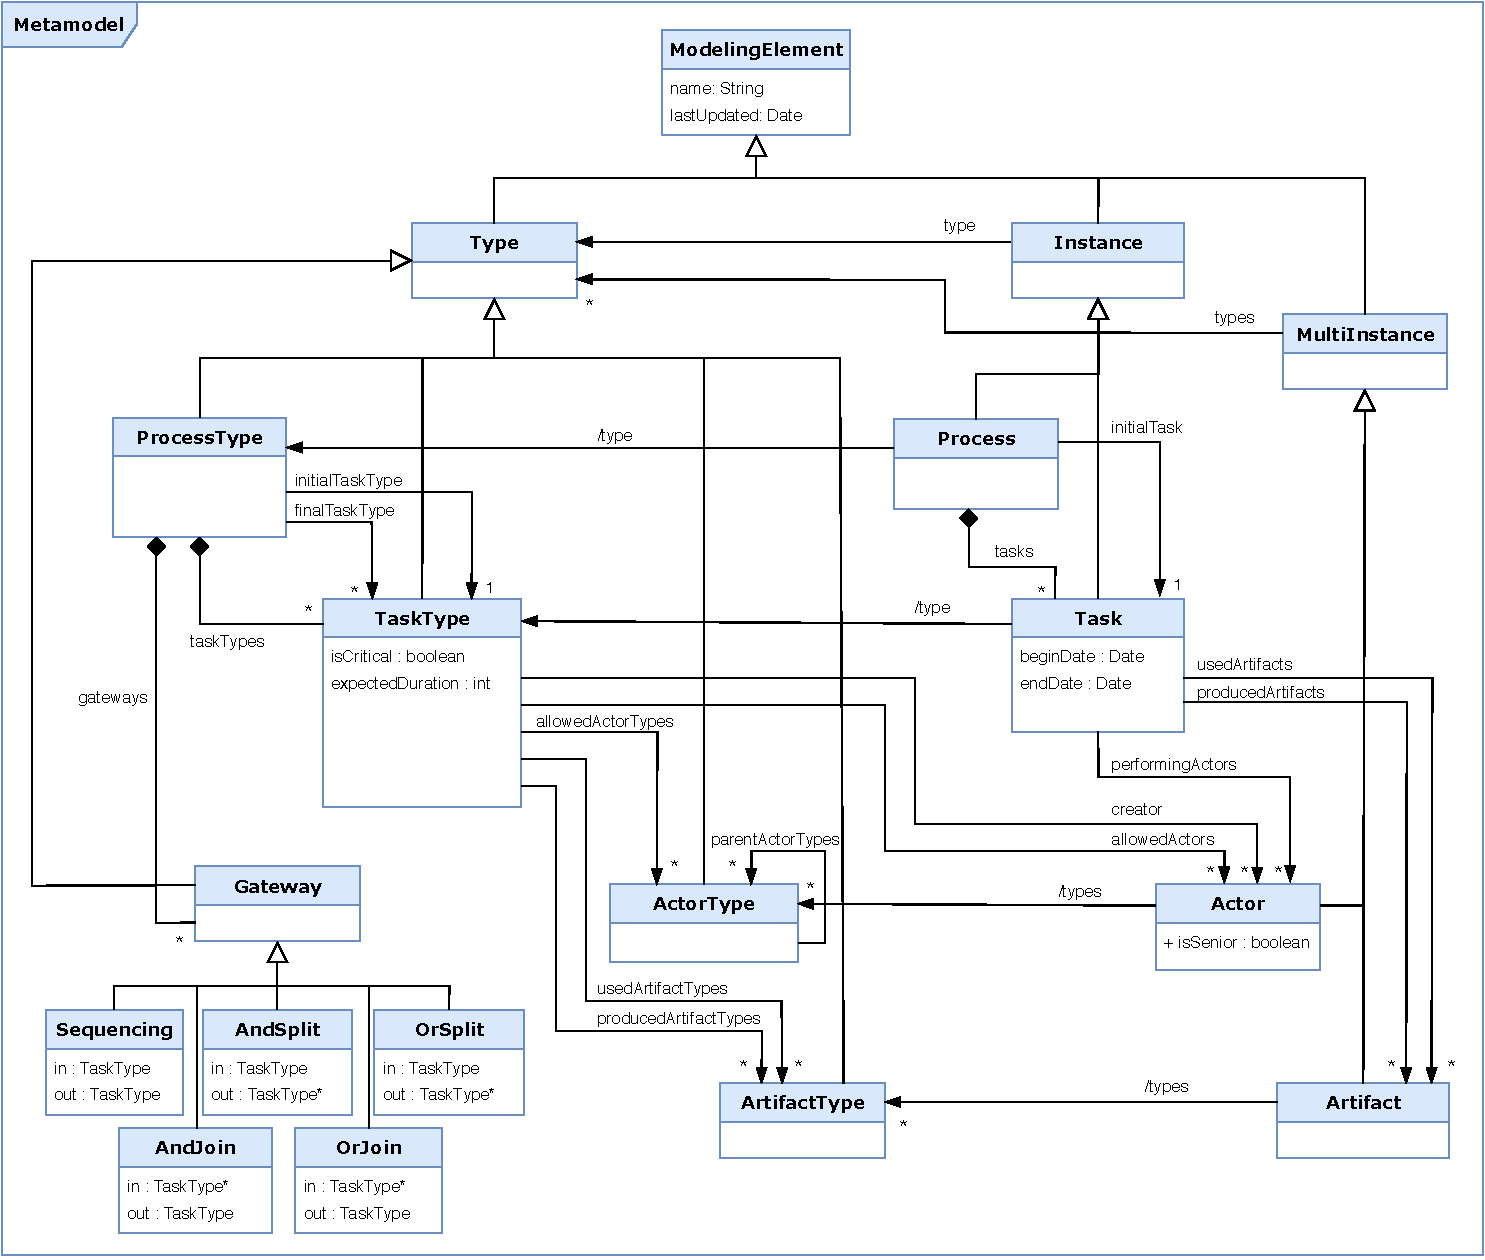
\includegraphics[width=1.0 \columnwidth]{Figures/Metamodel.pdf}
    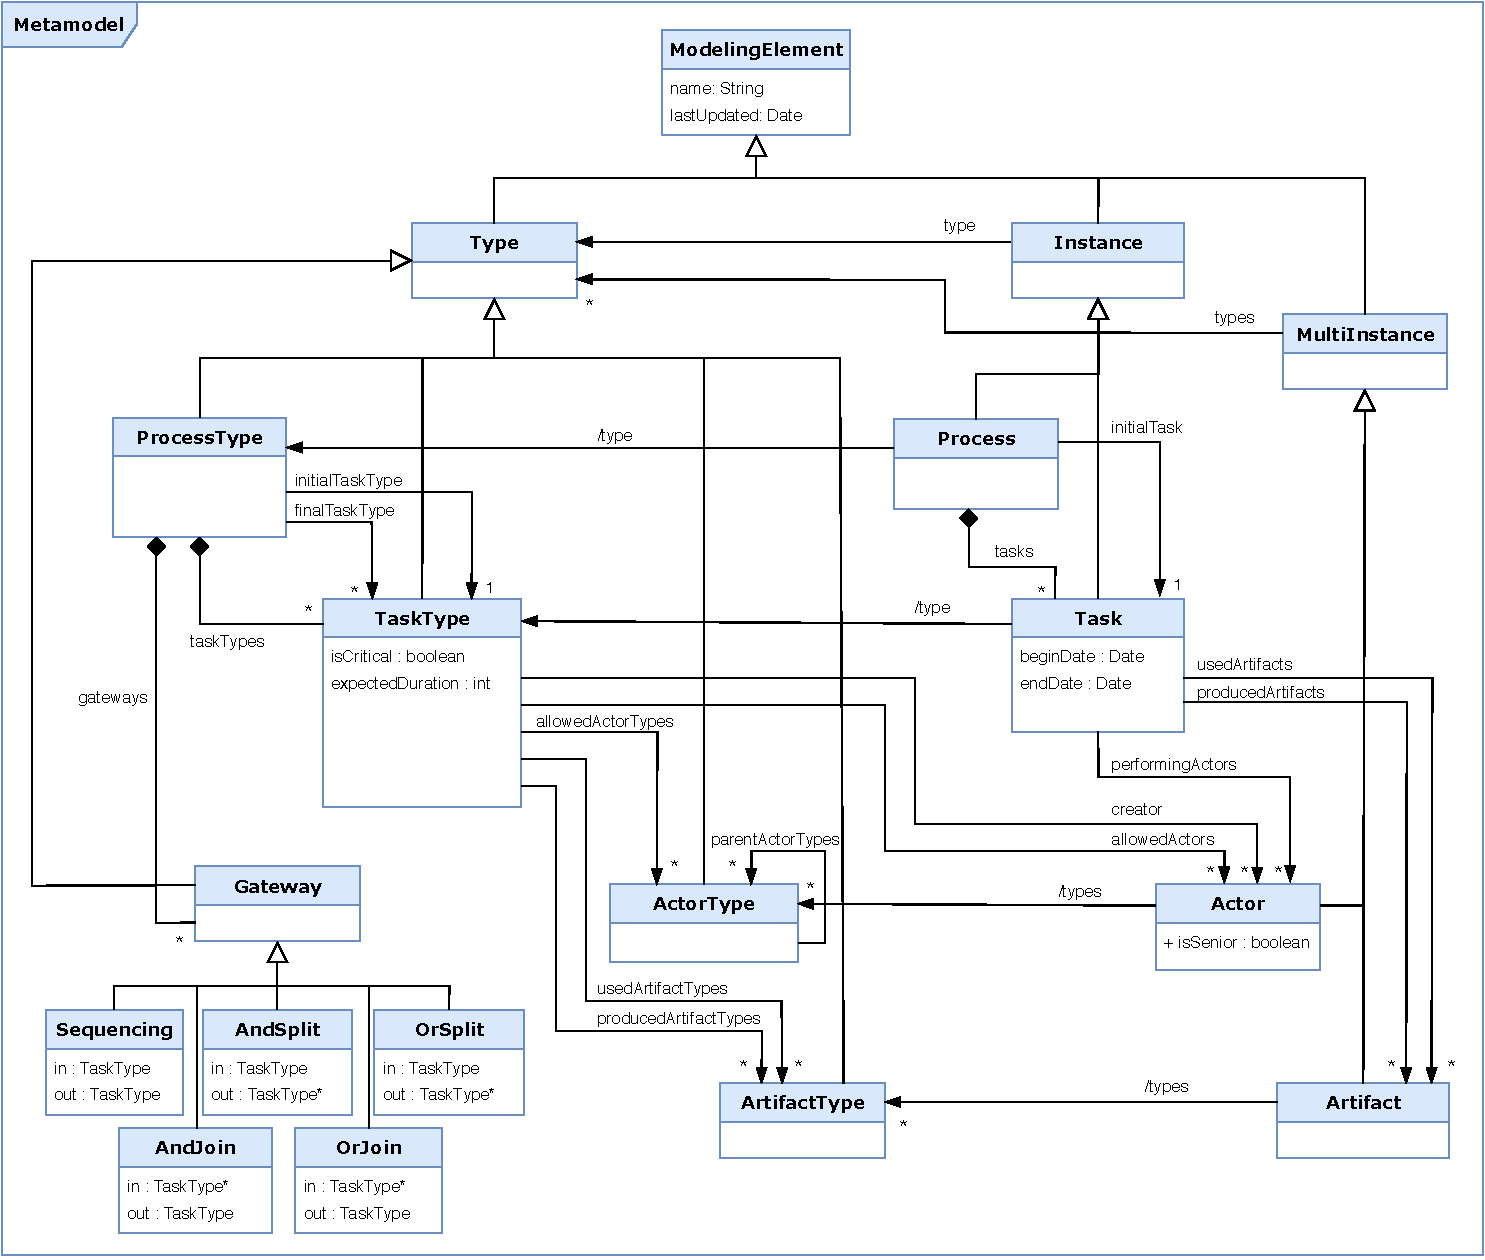
\includegraphics[width=1.0 \textwidth]{Figures/Metamodel.pdf}
     \caption{Process management base metamodel (\texttt{Gateway}'s associations with \texttt{TaskType} are represented with attributes)}
    \label{fig:BaseMetamodel}
\end{figure*}

In this section, we present the base metamodel presented in Figure~\ref{fig:BaseMetamodel} with the \textit{XSure} insurance domain use case, whose partial description was provided in the challenge description. The requirements \textbf{P1} to \textbf{P19} of XSure insurance domain are straightforwardly implemented by instantiating the \emph{XSure model}, as an instance of base metamodel (the left side of figure~\ref{fig:MultilevelArchitecture}).

Figure~\ref{fig:BaseMetamodel} represents this base metamodel with a \UML-like formalism, well adapted to represent \FML concepts and their instances. A \textit{Concept} of \FML is represented by a \UML class where roles of basic types are attributes. The roles whose types are concepts are represented by an arrow from their concept to their type, with their name on the arrow. The cardinality follows the \UML practice.
For example, the role \texttt{parentActorTypes} of the concept \texttt{ActorType} has the type \texttt{ActorType} and the * cardinality.

Our proposition relies on ontological instantiation as presented in figure \ref{fig:LinguisticAndOntologicInstantiation}, with a common root concept \texttt{ModelingElement}. Two types of ontological instantiation are needed to meet the requirements of the challenge. One provides that some instances conform to only one type (\texttt{Process} and \texttt{Task} do respectively conform to \texttt{ProcessType} and \texttt{TaskType}). While some entities define their conformity to several types (\texttt{Actor} and \texttt{Artifact} do respectively conform to several \texttt{ActorType} and \texttt{ArtifactType}). These instantiations are respectively expressed using the relations \texttt{type} and \texttt{types} between \texttt{Type}, \texttt{Instance} and \texttt{MultiInstance} concepts. In the diagram, the realization of these relations are indicated by a derived relation, \texttt{/type} or \texttt{/types}, as for example between \texttt{Process} and \texttt{ProcessType} or between \texttt{Actor} and \texttt{ActorType}.

\subsubsection{Process type definition}

We first present the process definition part of the base metamodel, located on the left of Figure \ref{fig:BaseMetamodel}.

% Illustrer avec des instances de XSure

\texttt{ProcessType} is a specialization of the \texttt{Type} concept, and references a collection of \texttt{TaskType} through the composition relation \texttt{taskTypes} with (0..*) cardinality (\textbf{P1}). A \texttt{TaskType} is embedded in a \texttt{ProcessType} and inherits from its context. To illustrate this in \textit{XSure} insurance domain use case, \textit{XSure model} defines \inst{Claim Handling}, instance of \texttt{ProcessType}, and \inst{Receive Claim}, \inst{Assess Claim} and \inst{Pay premium}, instances of \texttt{TaskType}.

\texttt{ProcessType} also references a collection of gateways, reified with the \texttt{Gateway} concept hierarchy. \texttt{Gateway} is a specialization of \texttt{Type} and is specialized by \texttt{Sequencing}, \texttt{AndSplit}, \texttt{AndJoin}, \texttt{OrSplit} and \texttt{OrJoin} concepts (\textbf{P2}). Depending on its type and following its underlying operational semantics, a gateway defines one or more inputs and one or more outputs. A \texttt{ProcessType} additionally exposes a unique initial \texttt{TaskType} and a collection of final \texttt{TaskType} with both roles \texttt{initialTaskType} (single cardinality) and \texttt{finalTaskType} (cardinality 0..*) (\textbf{P3}). \texttt{TaskType} exposes a creator role as a reference to an \texttt{Actor} concept (\textbf{P4}), which is at the same conceptual level.

The following listing shows an excerpt of the \FML code modeling some core concepts of the process modeling base metamodel.

\begin{lstlisting}
model MetaModel {

  concept ModelingElement { ... }

  concept Type extends ModelingElement { ... }

  concept ProcessType extends Type {
    TaskType[0..*] taskTypes;
    TaskType initialTaskType;
    TaskType[0..*] finalTaskTypes;
    Gateway[0..*] gateways;

    concept TaskType extends Type {
      Actor creator;
      Actor[0..*] allowedActors;
      ActorType[0..*] allowedActorTypes;
      ...
    }

    abstract concept Gateway extends Type {
      abstract void execute(Process process);
      ...
    }

    concept Sequencing extends Gateway {
      TaskType in;
      TaskType out;
    }

    // Other core concepts
  }
}
\end{lstlisting}


The \texttt{ActorType} concept inherits from the \texttt{Type} concept and the \texttt{allowedActorTypes} relation to \texttt{ActorType} defined in \texttt{TaskType} (with 0..* cardinality) captures \textbf{P5} requirement. Requirement \textbf{P6} is symmetrically satisfied with \texttt{allowedActors} relation to \texttt{Actor} also defined in \texttt{TaskType} (with 0..* cardinality). The same modeling pattern applies to \texttt{ArtefactType} also extending the concept \texttt{Type}, and both relations \texttt{usedArtifactTypes} and \texttt{producedArtifactTypes} defined in \texttt{TaskType} (\textbf{P7}). \texttt{TaskType} additionally exposes an \texttt{expectedDuration} role (expressed in number of days), satisfying \textbf{P8}.

The \texttt{Actor} concept defines a boolean attribute called \texttt{isSenior}, while \texttt{TaskType} defines an additional \texttt{isCritical} boolean attribute, indicating that some instances are flagged as critical and must be performed by senior actors. To fulfill \textbf{P9} requirement, a supplementary constraint is required for \texttt{TaskType} and is captured through the following invariant expressed in the \FML language:

\begin{lstlisting}
forEach (actor : allowedActors) {
    assert !isCritical | actor.isSenior
}
\end{lstlisting}

This invariant should be completed with additional constraints defined in the \texttt{Task} concept, which apply to performing actors assigned to enact tasks.

\subsubsection{Process enactment}
\label{sec:ProcessEnactment}
We now present the process enactment part of base metamodel, located right of figure~\ref{fig:BaseMetamodel}. All concepts defined in this subsection are either specializations of the \texttt{Instance} concept (if they have exactly one type) or the \texttt{MultiInstance} concept (when they have several types).

\texttt{Process} represents an enacted \texttt{ProcessType}, as defined in previous subsection (\textbf{P10}). \FML defines behavioral features called behavior. \texttt{ProcessType} defines the behavior \texttt{newProcess(String)}, taking the name of the process to enact as argument:

\begin{lstlisting}
public Process newProcess(String name) {
  Process newProcess = new Process(name,this);
  for (taskType : taskTypes) {
    Task newTask = taskType.newTask(newProcess.name+"-"+taskType.name),newProcess);
  }
  return newProcess;
}
\end{lstlisting}

This scheme relies on \FML dynamic binding mechanism to delegate to task types
the responsibility of instances creation. An instance of \texttt{Process}
references its unique type \texttt{ProcessType} by the specialized
\texttt{/type} role. Each instance of \texttt{TaskType} is ontologically
instantiated with a \texttt{Task} (\textbf{P11}), using the same factory
pattern where \texttt{TaskType} has the responsibility to manage the
ontological instantiation. A \texttt{Task} references its unique
\texttt{TaskType}, and defines a \texttt{begin date} and an \texttt{end date}
basic role (\textbf{P12}).

The used and produced artifacts are implemented by roles
\texttt{usedArtifacts}, \texttt{producedArtifacts} and
\texttt{performingActors} defined in \texttt{Task} (\textbf{P13}). An instance
of \texttt{Artifact} specializes \texttt{MultiInstance} and references a set of
\texttt{ArtifactType} through the specialized \texttt{/types} role
(\textbf{P14} and \textbf{P16}). Likewise, \texttt{Actor} specializes
\texttt{MultiInstance} and references a set of \texttt{ActorType} through the
specialized \texttt{/types} relation (\textbf{P15}).

The semantics is unclear relatively to the instantiation policy for artifacts.
In the requirements, nothing is explicitly stated about the link between the
\emph{artifact type} of a \emph{task type} and the types of the artifacts of a
corresponding task.  Here, we assume that task execution implies that for each
used and produced \emph{artifact type} defined in a related \emph{task type},
it exists at least one artifact of the right type. The following excerpt of
\FML code shows a partial implementation of this. We proceed likewise for
produced artifacts.

\begin{lstlisting}
concept Task extends Instance {
  ...
  boolean declaresRequiredUsedArtifacts() {
    for (artifactType : type.usedArtifactType) {
      boolean found = false;
      for (artifact : usedArtifacts) {
        if (artifact.isOfType(artifactType))
          found = true;
      }
      if (!found) return false;
    }
    return true;
  }
  ...
}
\end{lstlisting}

Authorization for an actor to perform a task (\textbf{P17}) is captured either by the role \texttt{allowedActors} or the role \texttt{allowedActorTypes} defined in \texttt{TaskType}. This mechanism is completed by the behaviors \texttt{isAuthorizedActor}, \texttt{isValidActor} and \texttt{isValidActorType} defined in \texttt{TaskType}:

\begin{lstlisting}
concept TaskType extends Type {
 ...
 // Check that an Actor is authorized to perform a task, using allowed Actor and ActorTypes
  boolean isAuthorizedActor(Actor actor) {
    for (actType : allowedActorTypes) {
      if (actor.hasActorType(actType))
        return this.isValidActorType(actType);
    }
    for (act : allowedActors) {
      if (actor == act)
        return this.isValidActor(actor);
    }
    return false;
  }

 // Check that an Actor may perform this TaskType (override when required)
  boolean isValidActor(Actor actor) {
    return true;
  }

 // Check that an ActorType may perform this TaskType (override when required)
  boolean isValidActorType(ActorType actorType) {
    return true;
  }
  ...
}
\end{lstlisting}

The \texttt{Task} concept delegates this authorization to its task type, as shown in the following \FML code:

\begin{lstlisting}
concept Task extends Instance {
  ...
  boolean isAuthorizedActor(Actor actor) {
    return type.isAuthorizedActor(actor);
  }
  ...
}
\end{lstlisting}

Enforcing those constraints is finally performed by the definition of this invariant in the \texttt{Task} concept:

\begin{lstlisting}
forEach (actor : performingActors) {
  assert isAuthorizedActor(actor);
}
\end{lstlisting}

The default behavior states that all actors and actor types are valid for all task types. This modeling scheme offers many extension points, by the redefinition of some behaviors in the inherited concepts (although none were required in the context of \emph{XSure} use case).

Actor types specialization is captured by the \texttt{parentActorTypes} relation defined in \texttt{ActorType} (\textbf{P18}). This is completed by both the definition of the \texttt{hasActorType(ActorType)} behavior in \texttt{Actor} and the recursive behavior \texttt{isOrSpecializes(ActorType)} in \texttt{ActorType}:

\begin{lstlisting}
concept ActorType extends Type {
  ActorType[0..*] parentActorTypes;
  ...
  boolean isOrSpecializes(ActorType actorType) {
    if (actorType == this)
      return true;
    for (p : parentActorTypes) {
      if (p.isOrSpecializes(actorType)
        return true;
    }
    return false;
  }
  ...
}

concept Actor extends MultiInstance {
  ...
  boolean hasActorType(ActorType actType) {
    for (type : types) {
      if (type.isOrSpecializes(actType))
        return true;
    }
    return false;
  }
  ...
}
\end{lstlisting}

Each concept inherits from \texttt{ModelingElement}, which defines a \texttt{lastUpdated} attribute with \texttt{Date} type, and thus satisfies \textbf{P19} requirement.

\subsection{The Acme software development process}
\label{sec:AcmeSoftwareDevelopmentProcess}

The challenge describes in a second part a Software engineering process for a fictional Acme company. The Base metamodel described previously is too generic to capture all domain-specific aspects of this use case. We chose to complete the architectural hierarchy with a specific virtual model, specific to the Acme software development process metamodel, shown in figure~\ref{fig:AcmeFullArchitecture}.
The \textit{Acme} metamodel specializes the Base metamodel, and \textit{Acme model} is an instance of the \textit{Acme} metamodel. The metamodel inheritance is implemented by virtual model's inheritance. Any instance of the Acme model is either an instance of a concept defined in the Base metamodel, or a concept defined in the specialized \textit{Acme} metamodel.
% FML follows a classical object-oriented semantics. ???

%\begin{figure}[t]
% \centering
%    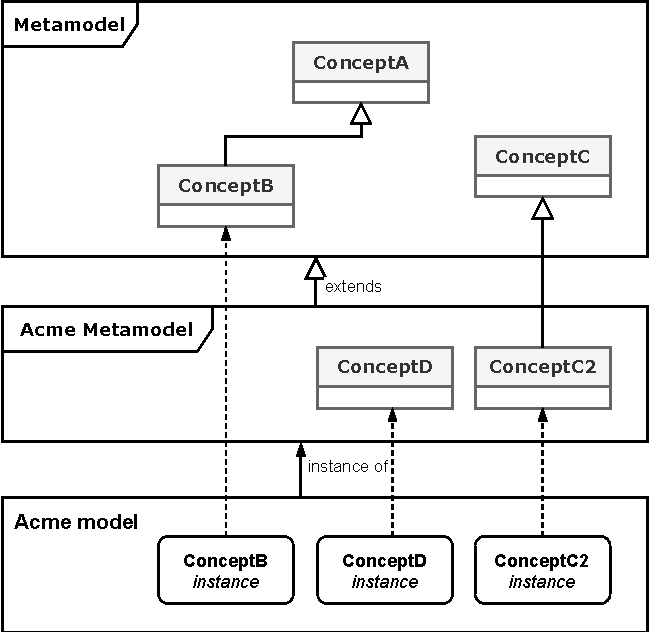
\includegraphics[width=1.0 \columnwidth]{Figures/AcmeArchitecture.pdf}
%     \caption{Acme software development process architecture}
%    \label{fig:AcmeArchitecture}
%\end{figure}

\begin{figure*}
 \centering
     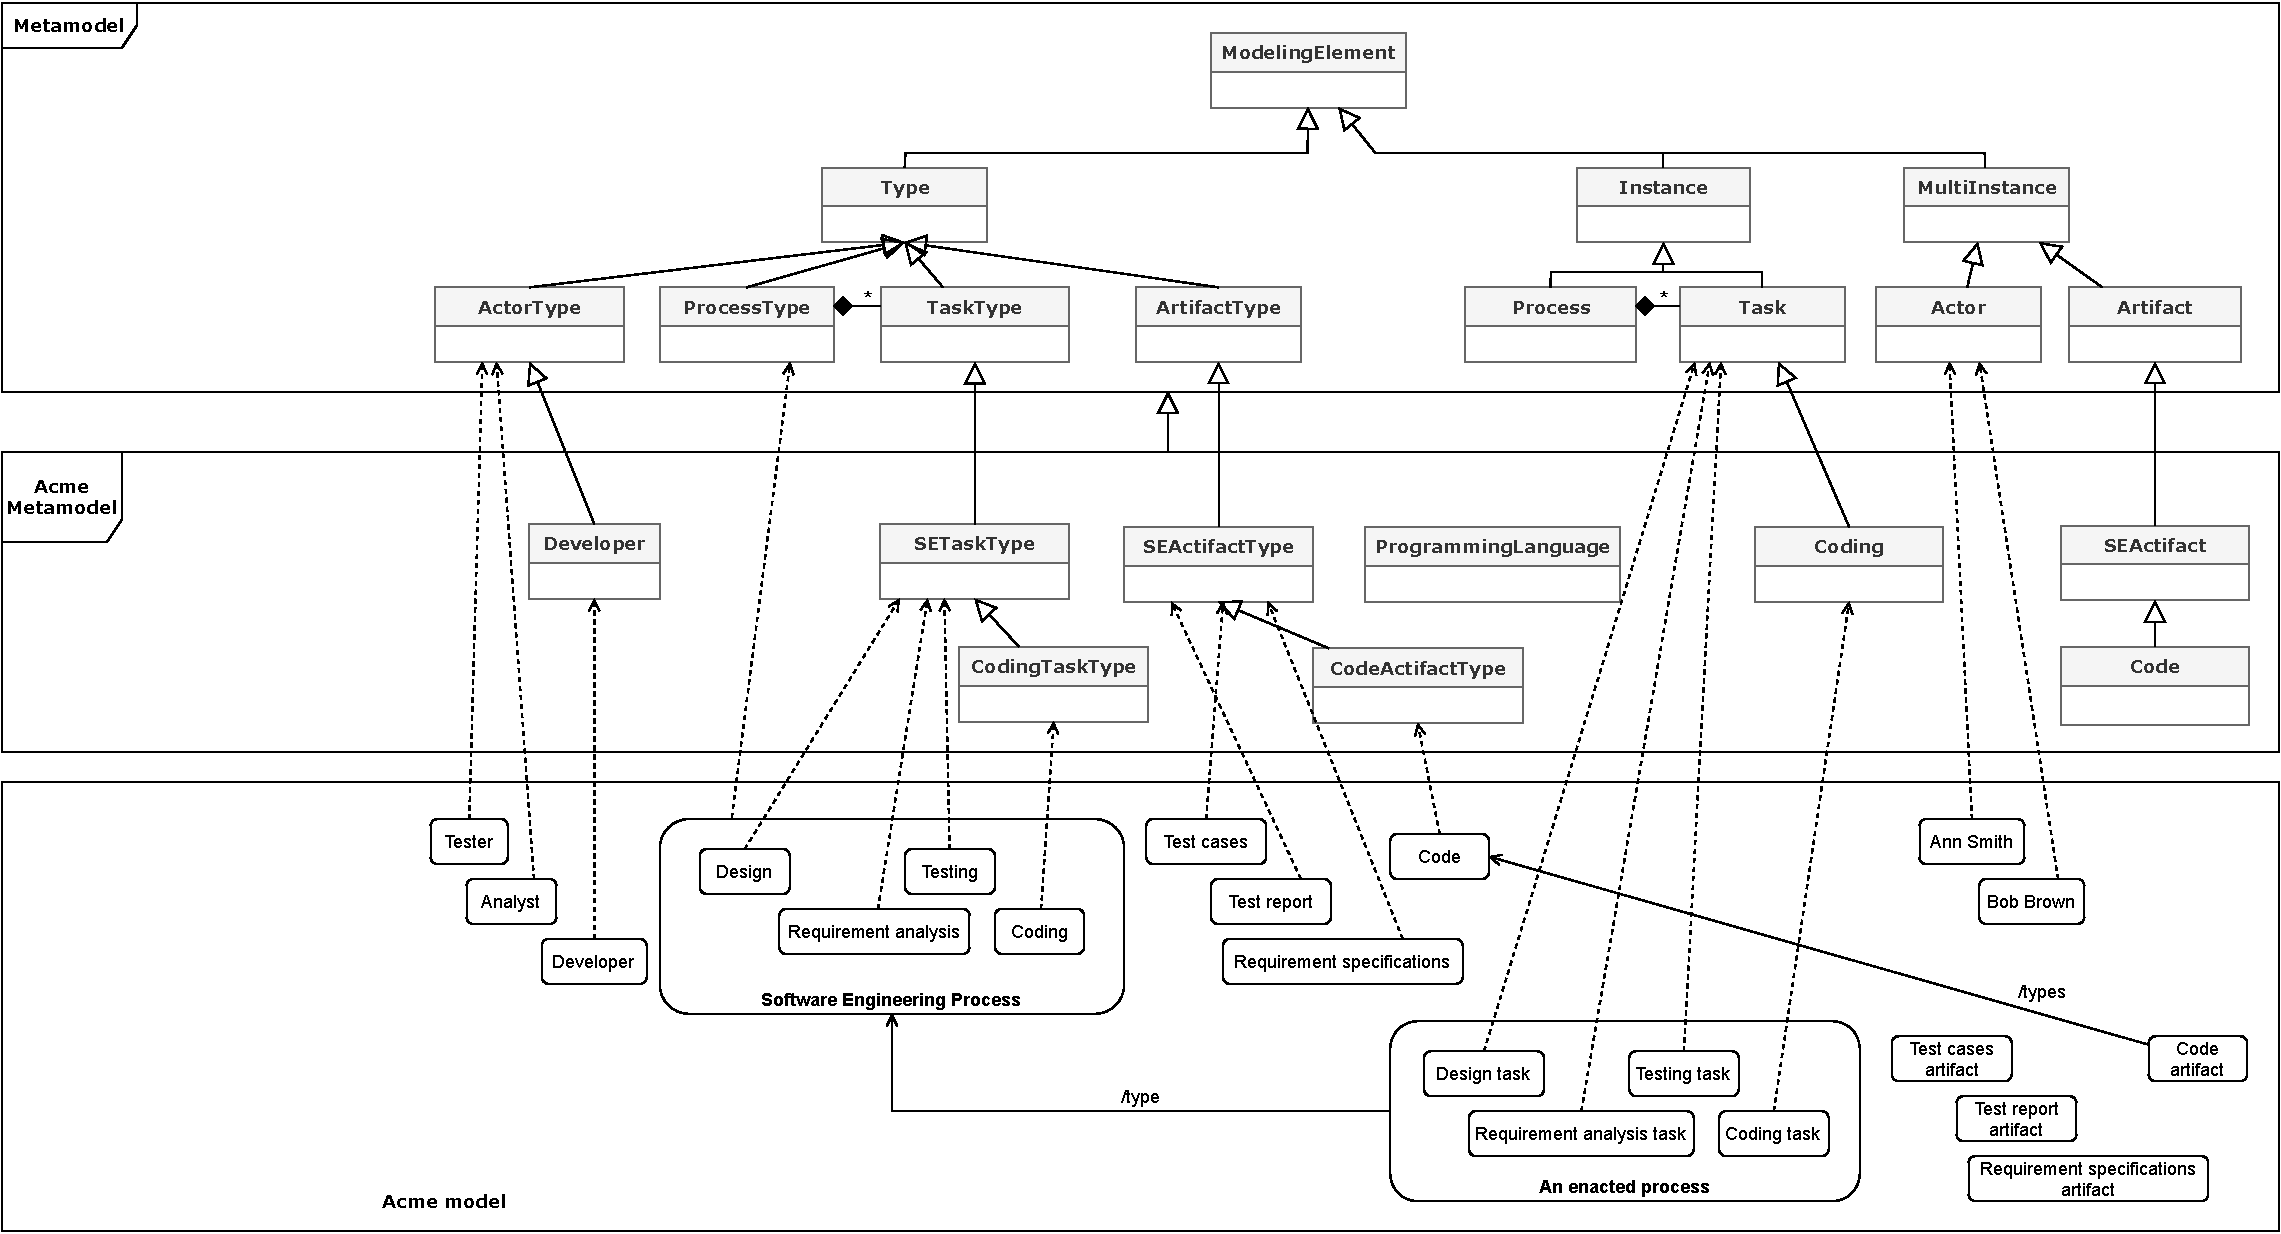
\includegraphics[width=1.0 \textwidth]{Figures/AcmeFullArchitecture.pdf}
     \caption{Acme software development process architecture (not all instances are shown for the sake of readability)}
    \label{fig:AcmeFullArchitecture}
\end{figure*}

The Figure~\ref{fig:AcmeFullArchitecture} highlights all conceptual levels of the architecture. This figure is only partial at instance level and not all instances are represented. It also contains an instance of enacted a \textit{Software Engineering Process} at the bottom. The Acme metamodel specializes some concepts of the Base metamodel, for example, \texttt{SETaskType} extends \texttt{TaskType} and \texttt{SEArtifactType} extends \texttt{ArtifactType}. These concepts are further specialized  \texttt{CodingTaskType} extends \texttt{SETaskType} and \texttt{CodeArtifactType} extends \texttt{SEArtifactType}.
The Acme metamodel also defines a specialized task type \texttt{Coding} extending \texttt{Task}, and provides the \texttt{Developer} concept extending \texttt{ActorType}. This metamodel is completed with the \texttt{ProgrammingLanguage} concept, defined as an enumeration (\texttt{Java}, \texttt{C}, \texttt{COBOL}). All the instances required to capture the challenge use case are defined in the final Acme model (lower part of the figure). Instances are represented with rounded boxes and linguistic instantiation is represented using dashed connectors.

The \textit{Software Development Process} for Acme company is presented in the figure~\ref{fig:AcmeSoftwareDevelopmentProcess}. It is a screen capture of the tool developed for the challenge and described in the next section.

\begin{figure}[t]
 \centering
    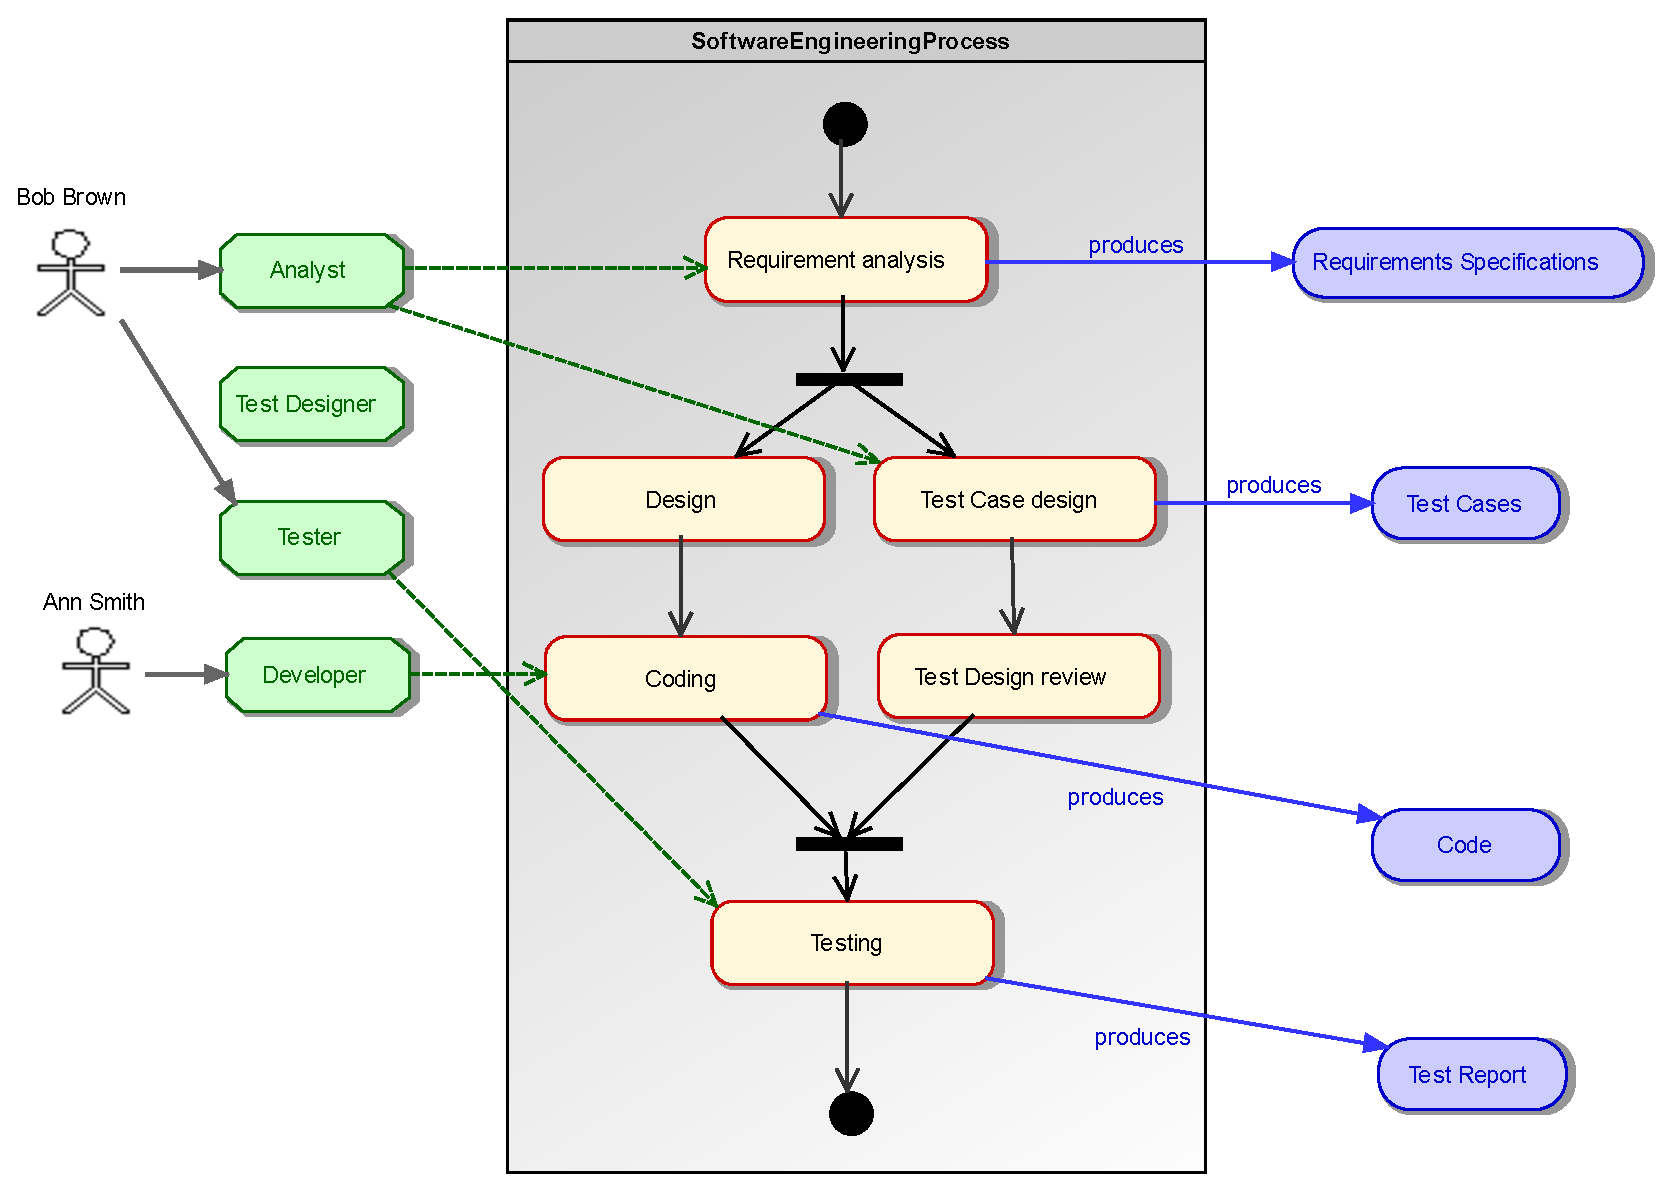
\includegraphics[width=1.0 \columnwidth]{Figures/SoftwareEngineeringProcessCroped.pdf}
     \caption{Acme software development process}
    \label{fig:AcmeSoftwareDevelopmentProcess}
\end{figure}

% J'utilise sf pour les instances et '

\inst{Requirements analysis} is an instance of \texttt{SETaskType}, \inst{Analyst} is an instance of \texttt{ActorType} and \inst{Requirement specifications} is an instance of \texttt{SEArtifactType}. The value of the property \texttt{producedArtifactTypes} of \inst{Requirements analysis} is \texttt{\{}\inst{Requirement specifications}\texttt{\}} and is \texttt{\{}\inst{Analyst}\texttt{\}} for \texttt{allowedActorTypes} (\textbf{S1}). Similarly, \inst{Test case design} is an instance of \texttt{SETaskType}, with a value of \texttt{true} for its property \texttt{isCritical}, and bound to \inst{Analyst} by the \texttt{allowedActorTypes} relation. \inst{Test case design} produces \inst{Test cases} instance of \texttt{SETaskType} (\textbf{S2}). The latter is used in \inst{Test design review} (\texttt{producedArtifactTypes} relation) (\textbf{S1} and \textbf{S13}, satisfied with \textbf{P9}).

The capture of \textbf{S3} requirement is performed while defining \inst{Coding} as an instance of concept \texttt{CodingTaskType} and defining a relation \texttt{languages} to \texttt{ProgrammingLanguage} with 1..* cardinality.
The \texttt{newTask(String)} behavior overrides the generic implementation by instantiating a \texttt{CodingTask} concept, specializing \texttt{Task}, as shown in the following excerpt of \FML code:

\begin{lstlisting}
concept CodingTaskType extends SETaskType {
  ProgrammingLanguage[1..*] languages;
  ...
  public CodingTask newTask(String name) {
    return new CodingTask(name,this);
  }
}
\end{lstlisting}

The \texttt{CodeArtifact} concept extends \texttt{SEArtifact}, and defines a relation \texttt{languages} to \texttt{ProgrammingLanguage} with 1..* cardinality (\textbf{S4}).

\textbf{S5} is more ambiguous as a task type \texttt{CodingTask} defines one or more programming languages but produces code which is expressed in one language only. This requirement is captured through the redefinition of the behavior \texttt{declaresRequiredProducedArtifacts} where programming language should also match.
\textbf{S6} is guaranteed though the \texttt{languages} relation defined in \texttt{CodeArtifact} and the following invariant declared in \texttt{CodeArtifact}:
\begin{lstlisting}
forEach (artifactType : types) {
  assert !(artifactType instanceof CodeArtifactType) | artifactType.doesImplement(languages)
}
\end{lstlisting}

\inst{Ann Smith} is the only one allowed to perform coding in COBOL (\textbf{S7}). This is implemented through the redefinition of \texttt{newTask(String)} in \texttt{CodingTaskType}:

\begin{lstlisting}
concept CodingTaskType extends SETaskType {
  ...
  public CodingTask newTask(String name) {
    CodingTask result = new CodingTask(name,this);
    if (languages.contains(ProgrammingLanguage.COBOL))
      result.addToPerformingActors(getActor("Ann Smith"));
    return result;
  }
}
\end{lstlisting}

The requirement \textbf{S8} is simply expressed by the definition of the \inst{Testing} instance of \texttt{SETaskType}, \inst{Tester} instance of \texttt{ActorType}, and \inst{Test report} instance of \texttt{ArtifactType}, as showed in the figure \ref{fig:AcmeSoftwareDevelopmentProcess}.

A critical task must additionally produce artifacts that must be associated with a validation task. This is modeled with a supplementary relation \texttt{validatedWith} defined in \texttt{Artifact} and referencing \texttt{Artifact} validating it (\textbf{S9}).

All software engineering artifacts defined in the context of Acme Software Engineering Process are  instances of \texttt{SEArtifact}. This concept defines two attributes: \texttt{responsible} (an \texttt{Actor} instance), and \texttt{versionNumber} (an integer). It thus fulfills \textbf{S10}. \inst{Bob Brown} is declared as an instance of \texttt{Actor}, and references \inst{Analyst} and \inst{Tester} (\texttt{ActorType} instances). He is also referenced by all instances of \texttt{SETaskType} as the creator for related task types (\textbf{S11}).


For \textbf{S12}, we assume that all tasks may define an expected duration, which might be checked during process execution. This is modeled by the \texttt{expectedDuration} attribute in \texttt{TaskType}. Alternatively, this could be modeled through the definition of a \texttt{SETesting} concept, as a specialization of \texttt{SETaskType}, and the instantiation of \inst{Testing} as an instance of \texttt{SETesting}. The business logic expressed by \textbf{S12} requirement should then be redefined in \texttt{SETesting}.

\textbf{S13} requirement has been previously partially fulfilled. This must be completed with an association between an artifact produced and the task that validates it. This is modeled by the reference to \inst{Test Cases} as a produced artifact type in \inst{Test Case design} and the reference to \inst{Test Cases} as a used artifact in \inst{Test Design review}, as shown in figure~\ref{fig:AcmeSoftwareDevelopmentProcess}.


\subsection{Openflexo tooling}
\label{subsec:tooling}

\begin{figure*}
 \centering
     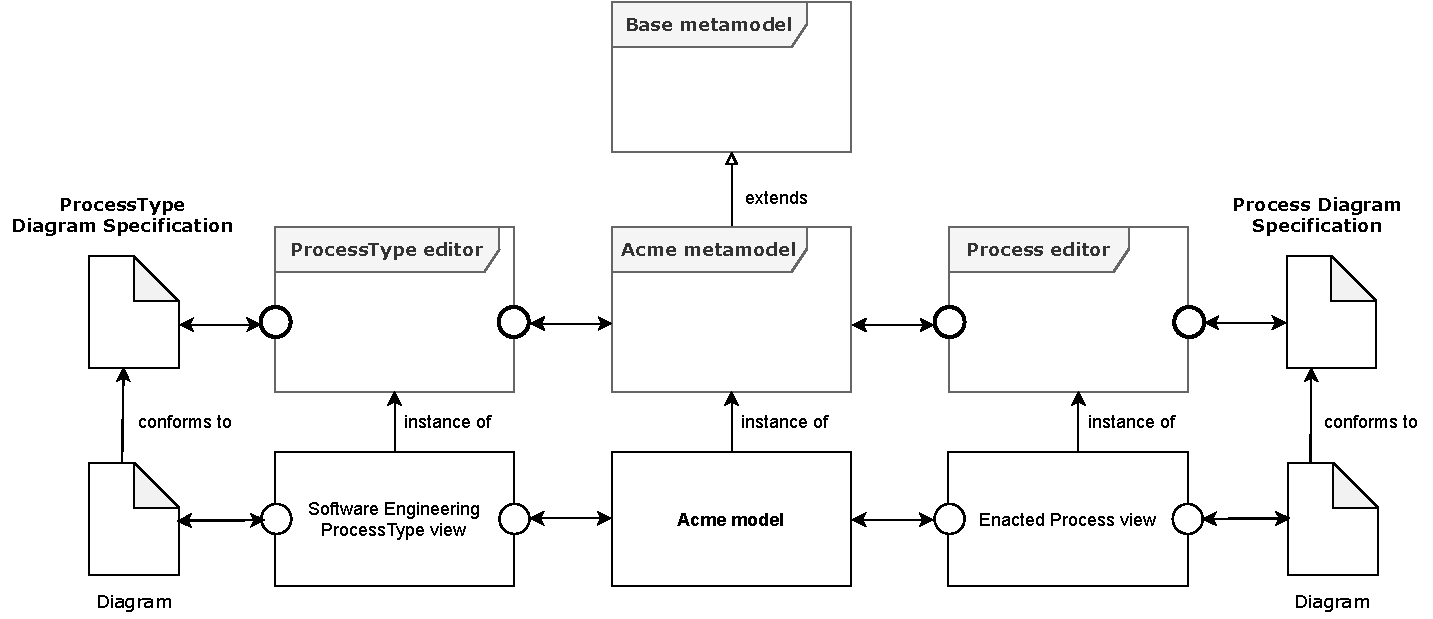
\includegraphics[width=0.9 \textwidth]{Figures/ToolingArchitecture.pdf}
     \caption{Tooling architecture}
    \label{fig:ToolingArchitecture}
\end{figure*}

\begin{figure*}
 \centering
     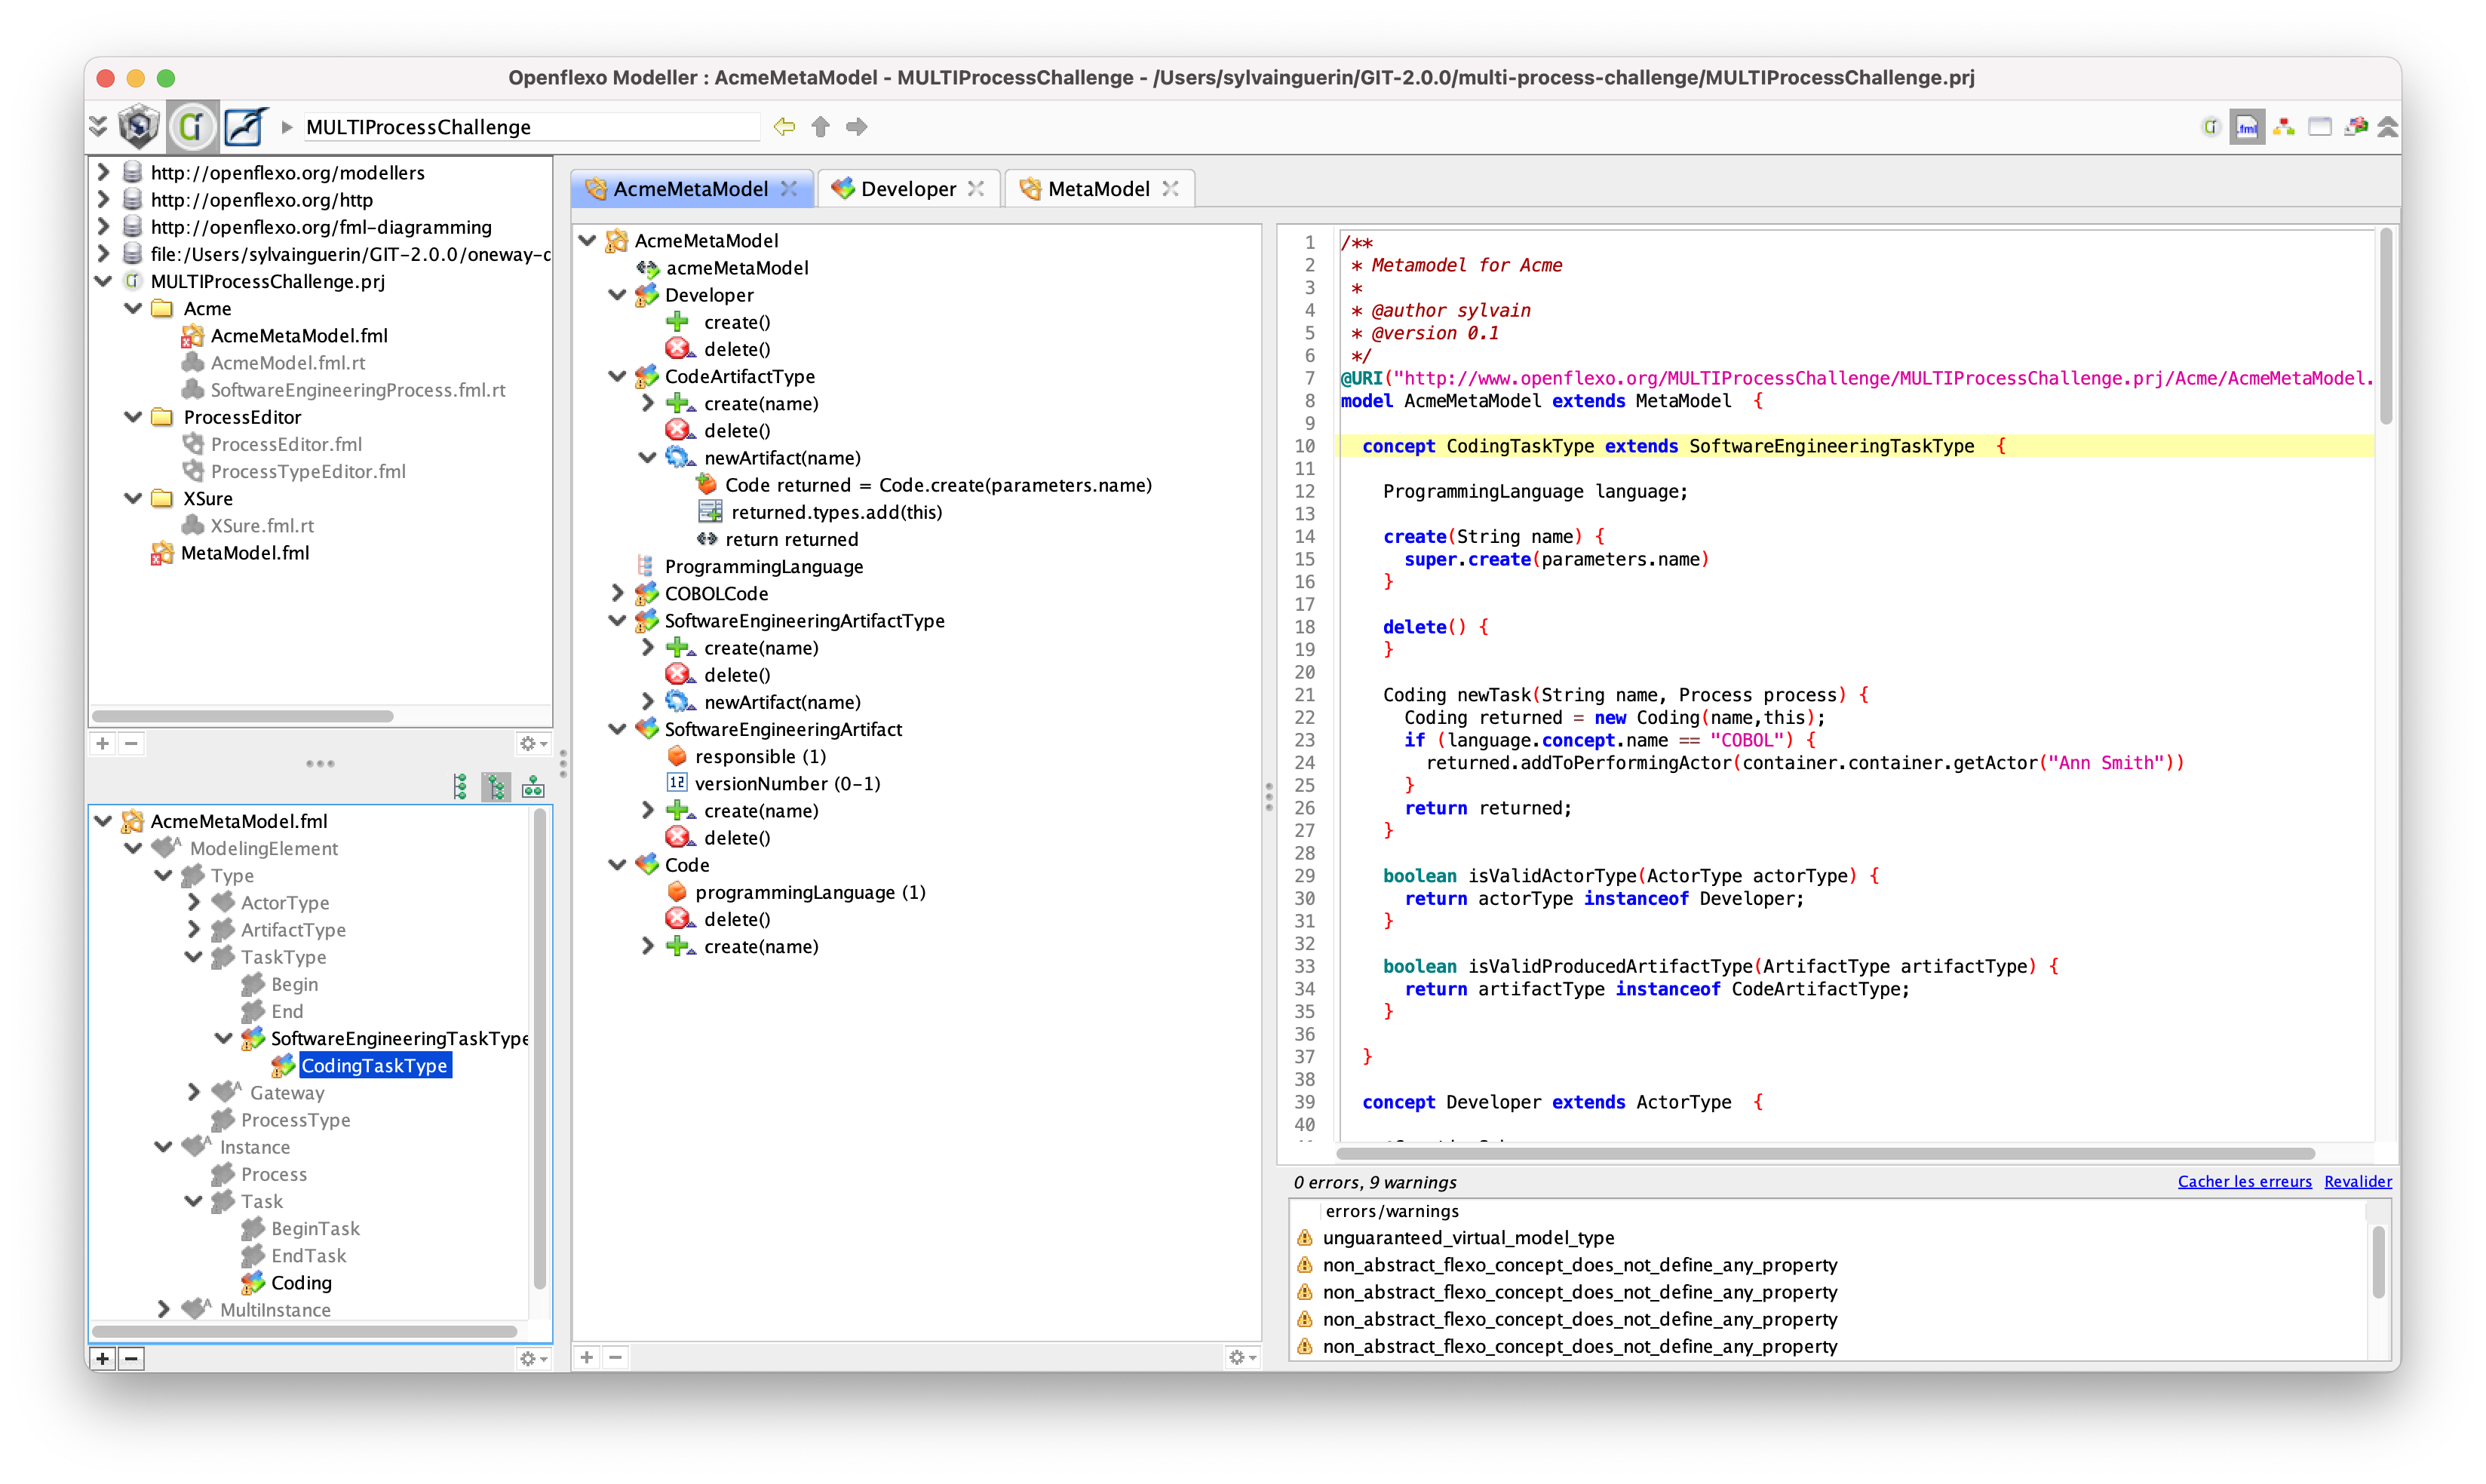
\includegraphics[width=\textwidth]{Figures/ScreenshotFMLEditor.png}
     \caption{Screenshot of the FML metamodel editor}
    \label{fig:ScreenshotFMLEditor}
\end{figure*}

\begin{figure*}
 \centering
     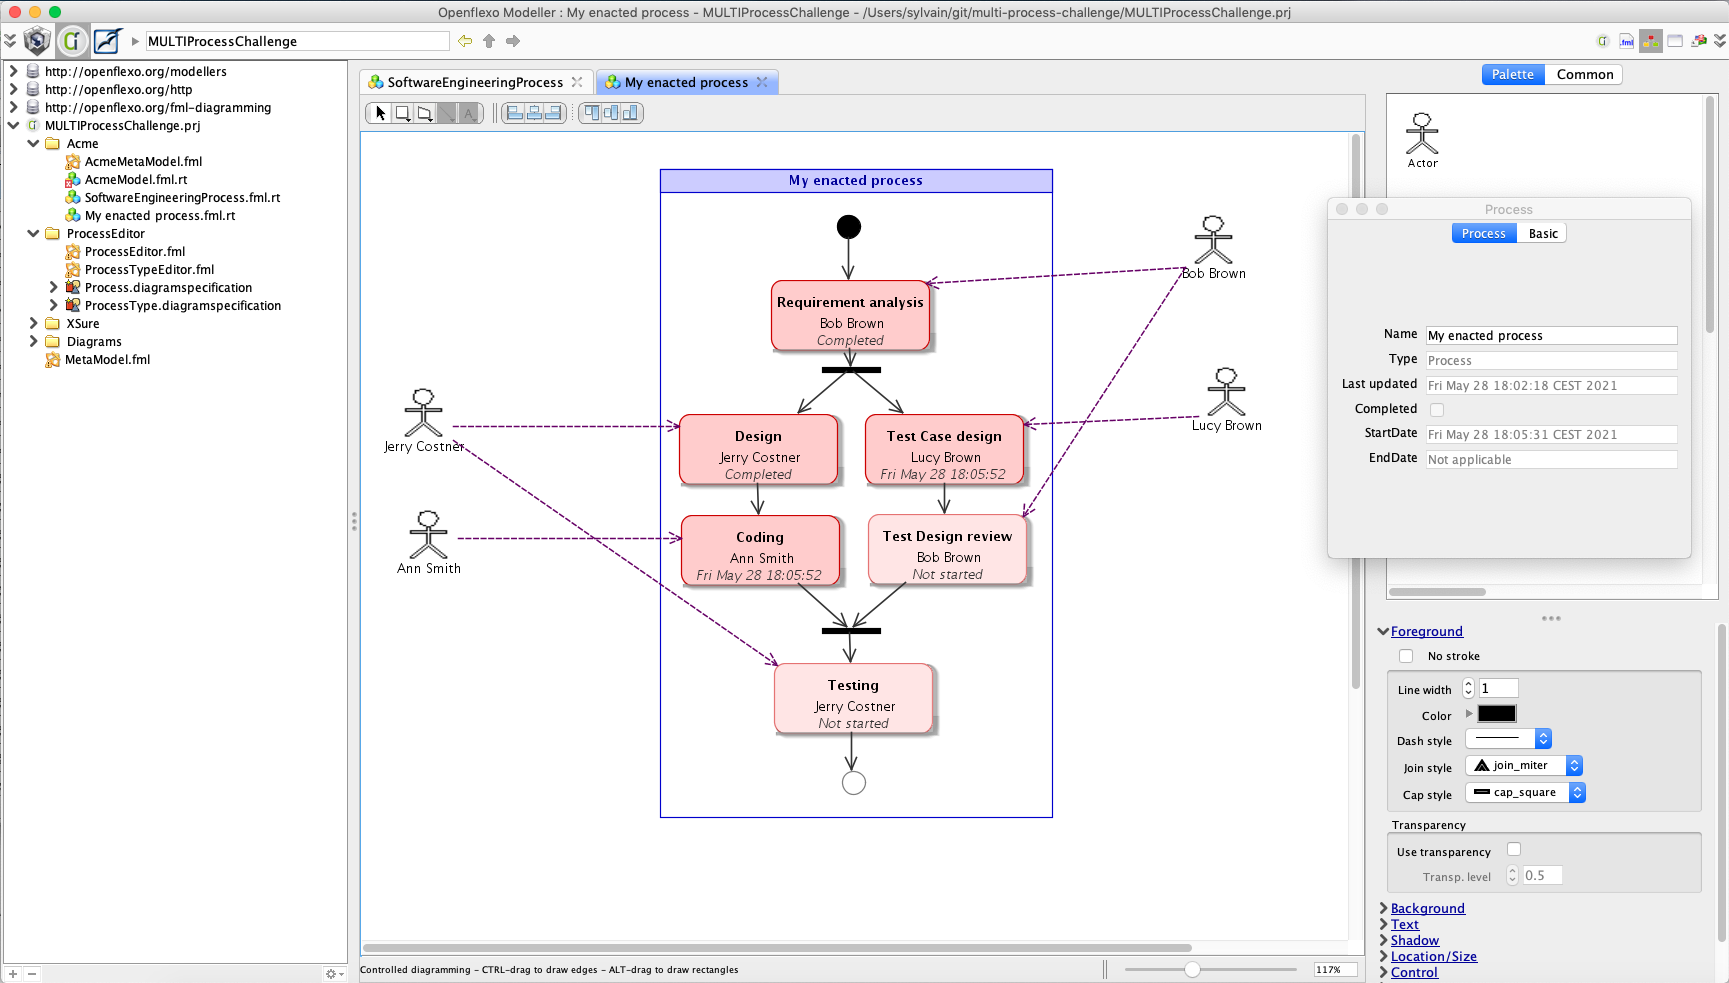
\includegraphics[width=\textwidth]{Figures/ScreenshotEnactedProcessEditor.png}
     \caption{Screenshot of the enacted process graphical editor}
    \label{fig:ScreenshotEnactedProcessEditor}
\end{figure*}

Our solution is fully implemented within the Openflexo tool. Both use cases have been modeled in the interactive design environment and can be executed by the \FML execution engine.


We took advantage of model federation and the availability of diagraming features though the \textit{Diagramming Technology Adapter} to implement two interactive graphical tools built on top of the conceptual levels detailed in previous sections. The figure \ref{fig:ToolingArchitecture} shows the overview of the tooling architecture and is detailed in the next section. A first tool offers a graphical edition of a Process type. The second one offers an enactment feature (the instantiation of a process from its process type), the ability within an enacted process to assign tasks to actors, and a graphical visualization of this process execution.


The Base metamodel is completed with some behaviors implementing an execution semantics for the executed processes. All tasks -- instantiated from \texttt{TaskType} for a given enacted process -- manage a status. This status is either \texttt{Not startable} (when not assigned to a performing actor or when required input artifacts are not available), \texttt{Startable}, \texttt{Started}, \texttt{Completable} (when all output artifacts are ready) or \texttt{Completed}. A \texttt{Task} also manages a set of performing actors, a begin and end date, some used and produced artifacts. The \texttt{Gateway} business logic has also been implemented through the implementation of an abstract \texttt{execute(Process)} behavior. The management of artifacts whose semantics follows rules defined in section~\ref{sec:ProcessEnactment} (\textbf{P13}) is also implemented.

Figure \ref{fig:ToolingArchitecture} details the architecture of these two tools.
 The left of the figure presents the \textit{ProcessType graphical editor}. \texttt{ProcessTypeEditor} is modeled as a virtual model declaring two model slots (represented with bold circles). The first model slot references an instance of Acme metamodel, while the second model slot references an instance of diagram, conforms to the \textit{ProcessType diagram specification}\footnote{a diagram "metamodel" which defines and specify structure and graphical representations for edited items}. When executed, this tool manages a graphical view for an instance of Acme metamodel (the \textit{Acme model}) and a specific \texttt{ProcessType} instance. This tool allows representing and editing a \texttt{ProcessType}. The highly reflective nature of \FML and its tooling should be noted. When the drag and drop interactor is applied for a new item, the tool allows choosing the concept type to be instantiated. For example, when a \texttt{TaskType} is created, the user must choose a concept inheriting from \texttt{TaskType} -- in Acme use case it can be \texttt{SETaskTask} or \texttt{CodingTaskType} or default value \texttt{TaskType}).

The other tool, called \textit{Enacted process graphical editor} and shown on figure~\ref{fig:ScreenshotEnactedProcessEditor}, provides process edition and tasks assignations through a graphical visualization displaying the process being executed. This tool is represented on the right side of the figure~\ref{fig:ToolingArchitecture}. It follows the same architecture pattern of the \textit{ProcessType graphical editor}, with two model slots referencing both the model and a diagram. Process enactment is operated from a \texttt{ProcessType}, and must be defined using a name identifying the newly instantiated process. All tasks are created from their \texttt{TaskType} definition, and required assignments apply (if for example \inst{Coding} \texttt{TaskType} defines COBOL as output programming language, the related task is automatically assigned to \inst{Ann Smith}). Each task has a status as well as a set of performing actors, a begin and end date, and used and produced artifacts.

A demonstrative video for the proposed tooling is available on our website\footnote{\url{https://research.openflexo.org/MLMChallenge.html}}, as well as download and installation instructions.
